%----------------------------------------------------------------------------------------
%	DOCUMENT CONFIGURATIONS
%----------------------------------------------------------------------------------------

\documentclass{article}

\usepackage[pdftex]{graphicx}
\usepackage{xcolor,listings}%color support for listings
\usepackage{minted}
\lstset{
	basicstyle=\footnotesize,
	numbers=left,
	numberstyle=\footnotesize,
	keywordstyle=\color{blue!70},
	commentstyle=\color{red!50!green!50!blue!50},
	stringstyle=\ttfamily, % typewriter type for strings
	frame=shadowbox,
	rulesepcolor=\color{red!20!green!20!blue!20},
	escapeinside=``,
	xleftmargin=2em,xrightmargin=2em, aboveskip=1em,
	breaklines=true             % sets automatic line breaking
}

\renewcommand{\arraystretch}{1.5}

\newmintedfile{sql}{tabsize=4,fontsize=\small}
\newminted{sql}{tabsize=4,fontsize=\small}
\newmintedfile{c}{tabsize=4,fontsize=\small}
\newminted{c}{tabsize=4,fontsize=\small}


\title{Working with raw format files} % Title
\author{Victor Moreno} % Author name
\date{\today} % Specify a date for the report


\begin{document}

\maketitle % Insert title, author, date
%\setlength\parindent{0pt} % Removes all indentation from paragraphs


\section{Objective}

This document describes the structure of the "raw" format files generated by the usage of the HPCAP2 driver as explained in~\cite{MorenoTFM2012}.





\section{File data structures}

A raw file is composed by a set of consecutive packets.
Each packet is preceded by its corresponding header which contains information related to the packet just as shown in Fig.\ref{Fig:rawformat}:

\begin{description}
	\item[Seconds] 4 bytes containing the seconds field of the packet timestamp.
	\item[Nanoseconds] 4 bytes containing the nanoseconds field of the packet timestamp.
	\item[Caplen] 2 bytes containing the amount of bytes of the packet included in the file.
	\item[Len] 2 bytes containing the real size of the packet.
\end{description}


\begin{figure}[h]
	\centering
	\begin{center}
		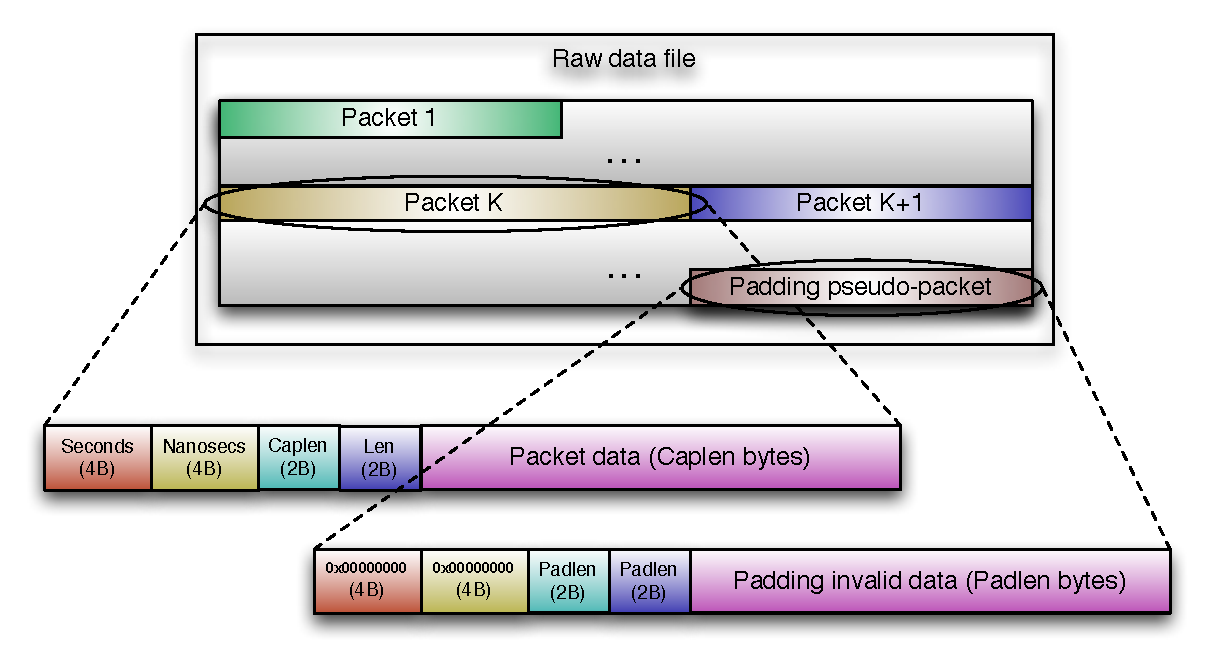
\includegraphics[angle=90,width=.9\textwidth]{figs/buff_raw2.pdf}
		\caption{Raw file format}
		\label{Fig:rawformat}
	\end{center}
\end{figure}


The end of the file is denoted by the appearance of a pseudo packet showing the amount of padding bytes added at the end of the file (in order to generate files of the same size).
The padding pseudo-packet has a similar header than any other packet in the file with the difference that both the "Seconds" and the "Nanoseconds" fields are set to zeros.
Once the padding pseudo-packet has been located, the padding size can be read from any of the "Len" or "Caplen" fields. Note that the padding length could be zero.


\section{Example code}

The next pages show an example code for a programs that reads a raw file and generates a new pcap file with the contents of the first one.

%\begin{itemize}
%\item[]
%\lstinputlisting[language=C,caption=Raw to PCAP conversion code,label=raw2pcap]{../samples/raw2/raw2pcap.c}
\cfile{../samples/raw2/raw2pcap.c}
%\end{itemize}

\bibliographystyle{unsrt}
\bibliography{hpcap_dpro10g}

\end{document}
